\chapter{Model-Based Fault Detection: Observer Approach}
\section{Introduction and Scope}
The functional safety layer presented in Chapter 5 relies on two primary detection mechanisms: \textbf{threshold-based monitoring} of the plant signals (torque and velocity) performed by the FaultMonitorMode plugin, and \textbf{communication watchdogs} that detect the loss of individual nodes or signal channels. These mechanisms are effective for a broad class of faults, particularly those that manifest as large, sustained deviations from the expected operating range or as complete signal loss. However, they are inherently limited in their ability to detect faults that produce subtle, gradual, or physically plausible signal corruptions — for instance, a slow drift in a force sensor calibration, a small but persistent bias in the encoder reading, or an incipient degradation of the actuator torque constant. In such cases, the corrupted signal may remain within the nominal threshold bounds while still causing a progressive deterioration of the control performance and, ultimately, of the safety of the interaction.

\textbf{Model-based fault detection} addresses this limitation by exploiting the availability of a physics-based model of the system — in this case, the reduced-order dynamic model of the exoskeleton described in Chapter 3 — to generate residual signals that are nominally zero when the system behaves according to the model and deviate from zero when a discrepancy arises between the predicted and the measured behavior. Because the residuals are sensitive to the internal consistency of the system rather than to the absolute magnitude of the signals, they can detect faults that are invisible to threshold-based monitors.

This chapter presents the observer-based fault detection module developed for the Digital Twin, implemented as the \textbf{exoskeletron\_observers} package. The module comprises four complementary detection layers - a Luenberger state observer, an admittance inversion estimator, a generalized momentum observer, and a rate-of-change guard - each targeting a different class of faults and operating at a different detection timescale.

It is important to clarify the scope and maturity level of this work. The observer module was developed as a secondary-or even tertiary-contribution within the broader context of the thesis, whose primary focus is the Digital Twin architecture, the constrained dynamic modeling, and the functional safety state machine described in the preceding chapters. Nonetheless, the observer node is fully implemented, operational, and integrated into the Digital Twin launch system: it runs at 200-Hz alongside the plant, controllers, and safety nodes, subscribes to the relevant topics, and publishes residual signals in real time. It has been used in conjunction with the fault injection framework of Chapter 5 to qualitatively verify that the residuals respond to injected faults on the expected channels and with the expected latencies.

However, the observer has not yet been connected to the safety decision chain: it publishes diagnostic residuals on dedicated topics but does not trigger any state transition in the safety state machine. The calibration of detection thresholds, the design of a formal decision logic (e.g., CUSUM, GLR, or voting-based schemes), and the integration with the \textbf{SENSOR\_DEGRADED\_MODE} state reserved in the safety architecture (Section 5.3.1) remain as future work. The following sections describe the theoretical foundation, the implementation, and the current capabilities and limitations of the observer module, as well as the envisioned integration path.


\section{Theoretical Background}
This section provides a \textbf{concise} overview of the observer-based fault detection concepts that underpin the implementation described in Section 6.3. The treatment is intentionally brief and focused on the specific formulations adopted in this work; the reader is referred to the established literature on model-based fault diagnosis for a comprehensive theoretical treatment.

\subsection{Observer-Based Residual Generation}
The fundamental idea of observer-based fault detection is to \textbf{compare the measured behavior of a system against the behavior predicted by a mathematical model}. An \textbf{observer} is a dynamic system that receives the same inputs as the real plant (actuator commands, known disturbances) and a subset of the measured outputs (sensor readings), and produces an estimate of the plant state. The difference between the measured output and the observer's predicted output is called the \textbf{residual} or \textbf{innovation}.

Under nominal conditions - when the plant behaves exactly as the model predicts and all sensors are functioning correctly - the residual converges to zero (or to a small value determined by modeling uncertainties and measurement noise). When a fault occurs, the discrepancy between the real plant and the model causes the residual to deviate from zero in a manner that is characteristic of the fault type, location, and magnitude.

\begin{figure}[ht]
    \centering
    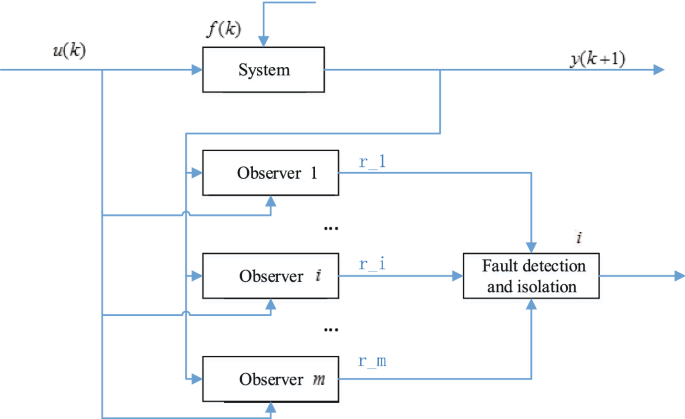
\includegraphics[scale=0.5]{images/chapter6/FDI_diagram.png}
    \caption{General architecture of observer-based fault detection and isolation (adapted from \cite{fault_detection_basic_info}).}
    \label{fig:FDI_diagram}
\end{figure}
\FloatBarrier

The quality of the fault detection depends critically on two factors: the \textbf{accuracy of the model} (which determines the nominal residual level) and the \textbf{sensitivity of the observer structure} to the fault of interest (which determines the signal-to-noise ratio of the residual under fault conditions). In the context of the hand exoskeleton Digital Twin, the reduced-order dynamic model of Chapter 3 provides a high-fidelity representation of the plant dynamics projected onto the crank coordinate $\theta$, including inertial, gravitational, Coriolis, friction, and passive biomechanical effects. This model is well suited for observer design because it is scalar (1-DOF), computationally inexpensive, and its parameters are shared with the dynamic simulation node, ensuring consistency between the plant and the observer.

\subsection{Luenberger Observer}
The Luenberger observer\cite{Luenberger1964_Observing} is the classical state estimation structure for linear and mildly nonlinear systems. For the reduced exoskeleton model, the state vector consists of the crank angle and its time derivative, $x = [\theta, \dot{\theta}]^T$, and the observer takes the form:

\begin{equation}
    \dot{\hat{x}} = f(\hat{x}, u) + L(y - \hat{y})
\end{equation}

where $f(\cdot)$ is the nonlinear plant model (the same reduced dynamic equation used in the simulation node), $u$ is the known input (motor torque, passive torques, external force estimate), $y$ is the measured output (encoder reading), $\hat{y}$ is the observer's predicted output (computed from $\hat{x}$), and $L = [l_1, l_2]^T$ is the observer gain matrix.

The gains are designed through pole placement: the desired poles of the observer error dynamics are specified, and the gains are computed such that the linearized error system has eigenvalues at the desired locations. For the reduced exoskeleton model, the linearized error dynamics around a given operating point can be approximated as a second-order system with a single damping parameter $D/M_{eff}$, where $D$ is the total linear dissipation coefficient and $M_{eff}$ is the effective inertia. The observer gains are then:

\begin{equation}
    l_1 = - (p_1 + p_2) - \frac{D}{M_{eff}}, \qquad l_2 = p_1 p_2 - l_1 \frac{D}{M_{eff}}
\end{equation}

where $p_1$ and $p_2$ are the desired observer poles. The choice of pole locations is a trade-off between convergence speed (faster poles) and noise sensitivity (slower poles). A practical constraint arises from the explicit Euler integration used in the implementation: with an integration step of $\Delta t = 5ms$ the pole magnitudes should remain below  50 to avoid numerical instability. The default values of $p_1 = -15$ and $p_2 = -20$ satisfy this constraint while providing convergence approximately 2–3 times faster than the dominant plant pole ($\lambda \approx -6$).

The residual - the innovation signal $r = \theta_{meas} - \hat{\theta}$ - is sensitive to any discrepancy between the model prediction and the measurement. In particular, faults on the position encoder (channel 3 in the fault injection framework) produce a direct, immediate effect on the innovation, making the Luenberger observer well suited for encoder fault detection.

\subsection{Generalized Momentum Observer}
The generalized momentum observer\cite{GMO_FaultDetection}, originally proposed for collision detection in robotic manipulators, provides an alternative residual generation approach that avoids the need to compute the joint acceleration $\ddot{\theta}$, a quantity that would require numerical differentiation of a noisy velocity signal.

The key insight is to work with the generalized momentum $p = M(\theta) \dot{\theta}$, rather than with the acceleration. The time derivative of the momentum can be expressed as:

\begin{equation}
    \dot{p} = M(\theta) \ddot{\theta} + \dot{M}(\theta) \dot{\theta} = \tau_{known} + \tau_{unknown}
\end{equation}

where $\tau_{known}$ groups all the torque contributions that can be computed from known signals (motor torque, passive torques, friction, projected nonlinear terms, measured external force) and $\tau_{unknown}$ represents unmodeled or unmeasured disturbances — including the effect of a sensor fault.

The observer introduces an auxiliary variable $\sigma$ that integrates the known terms plus a correction:

\begin{equation}
    \dot{\sigma} = \tau_{\text{known}} + r_{\text{mom}}, \qquad \sigma(0) = p(0)
\end{equation}
\begin{equation}
    r_{\text{mom}} = K_{\text{mom}} \cdot (p - \sigma)
\end{equation}

where $K_{\text{mom}}$ is a scalar gain. In steady state, the residual $r_{\text{mom}}$ converges to $\tau_{\text{unknown}}$, which under nominal conditions is zero. When a fault introduces a discrepancy — for example, an offset on the measured external force — $r_{\text{mom}}$ converges to the magnitude of the discrepancy with a time constant of approximately $1/K_{\text{mom}}$.

A practical advantage of this formulation is that the configuration-dependent variation of the effective inertia ($\dot{M}_{\text{eff}} \cdot \dot{\theta}$) can be compensated numerically without computing a continuous derivative:

\begin{equation}
    \Delta p_M \approx (M_{\text{eff},k} - M_{\text{eff},k-1}) \cdot \dot{\theta}
\end{equation}

This discrete compensation, applied at each integration step, absorbs the inertia variation into the integrator update and prevents it from appearing as a spurious residual.

\subsection{Rate-of-Change Monitoring}
The final detection layer is not model-based in the traditional sense but \textbf{exploits a physical constraint} on the external force signal. A force applied by a human hand to the exoskeleton is bounded in its rate of change by the biomechanical properties of the musculoskeletal system: muscle activation dynamics, tissue compliance, and limb inertia impose a physiological bandwidth of approximately 5-10 Hz on voluntary force production. This translates to a maximum rate of change on the order of 5-20 Nm/s for the force magnitudes relevant to hand rehabilitation.
 
By contrast, a fault-induced signal corruption - such as a step offset injected by a sensor malfunction or a communication error - produces an effectively instantaneous change in the measured force, with a rate of change that exceeds the physiological limit by one to two orders of magnitude. A 2 Nm offset appearing in a single 5 ms sample, for example, corresponds to a rate of 400 Nm/s.
 
The rate-of-change monitor computes the discrete derivative of the external force signal and compares its absolute value against a configurable threshold:

\begin{equation}
    \left| \frac{\Delta \tau_{\text{ext}}}{\Delta t} \right| = \left| \frac{\tau_{\text{ext},k} - \tau_{\text{ext},k-1}}{\Delta t} \right| \stackrel{?}{>} R_{\text{max}}
\end{equation}

With the default threshold $R_{\text{max}} = 100\,\text{Nm/s}$, the monitor provides a wide margin above the physiological range while remaining sensitive to sudden artificial transients. The detection latency is effectively one sample (5 ms), making this the fastest detection layer. Its primary limitation is that it is completely insensitive to slow drifts or gradual bias accumulation - faults that are instead well covered by the momentum observer.

\subsection{Complementarity of the Four Layers}
The four detection layers are designed to provide \textbf{complementary coverage} of the fault space rather than redundant detection of the same fault class. Each layer has a distinct sensitivity profile: the Luenberger observer is most sensitive to encoder faults; the admittance inversion is most sensitive to external force sensor faults; the momentum observer provides fast, broad-spectrum detection of torque-related discrepancies; and the rate-of-change guard provides instantaneous detection of impulsive signal corruptions. This complementarity is discussed further in Section 6.4, where the sensitivity and latency characteristics of each layer are summarized.


\section{Implementation}
The four detection layers described in the preceding section are implemented within a single ROS 2 node, \textbf{ObserverNode}, in the \textbf{exoskeletron\_observers} package. The node runs at 200 Hz - the same rate as the dynamic plant and the control loop - and subscribes to five topics: the joint state feedback (\textbf{/joint\_states}), the measured external force (\textbf{/exo\_dynamics/tau\_ext\_theta}), the feed-forward dynamic terms (\textbf{/exo\_dynamics/ff\_terms}), the raw torque command \newline(\textbf{/torque\_raw}), and the trajectory reference (\textbf{/trajectory\_ref}). At each update cycle, all four detection layers are evaluated and their residuals are published on dedicated topics for logging and monitoring.

The node waits until all five subscriptions have received at least one message before beginning the update loop, ensuring that no observer operates on stale or default-initialized data. All plant model parameters - friction coefficients, damping, and the Coulomb threshold - are declared as ROS 2 parameters and loaded from the \textbf{observer\_params.yaml} configuration file, which mirrors the values used by the dynamic simulation node to ensure model consistency.

\subsection{Observer 1 - Luenberger State Observer}
The Luenberger observer maintains an internal estimate of the crank state $(\theta, \dot{\hat{\theta}})$ and updates it at each cycle using the full nonlinear plant model augmented by a correction term proportional to the position innovation. The prediction step computes the expected angular acceleration from the known inputs - motor torque, passive biomechanical torque, external force estimate, projected nonlinear terms, and dissipative effects - using the same reduced dynamic equation implemented in the plant node:

\begin{minted}{python}

tau_fric_visc = fric_visc * self._theta_dot_hat
tau_fric_coul = fric_coul * math.tanh(self._theta_dot_hat / fric_eps)
tau_damp = damping * self._theta_dot_hat
tau_dissipative = tau_fric_visc + tau_fric_coul + tau_damp

theta_ddot_model = (
    self._tau_m
    + self._tau_pass
    + self._tau_ext_meas
    - self._proj
    - tau_dissipative
) / self._M_eff

\end{minted}

The correction step applies the Luenberger gains $l_1$ and $l_2$ to the position innovation $e = \theta - \hat{\theta}$, and the state is propagated forward using explicit Euler integration:

\begin{minted}{python}

innov = self._theta_meas - self._theta_hat

theta_dot_hat_new = (
    self._theta_dot_hat
    + dt * (theta_ddot_model + l2 * innov)
)
theta_hat_new = (
    self._theta_hat
    + dt * (self._theta_dot_hat + l1 * innov)
)

\end{minted}

The gains are computed from the desired observer poles $p_1$ and $p_2$, using the formulas derived in Section 6.2.2. The default pole placement results in gains $l_1 = 29$ and $l_2 = 126$ for the nominal plant parameters. The positive value of $l_1$ is correct and expected: it ensures that a positive innovation (measured position ahead of the estimate) accelerates the position estimate, reducing the error.

The \textbf{state residual} - the innovation signal $r = \theta_{meas} - \hat{\theta}$ -  is published on
\textbf{/observer/state\_residual} at every cycle. Under nominal conditions, this residual remains close to zero after the initial convergence transient. A fault on the position encoder (channel 3 in the fault injection framework) produces a direct, immediate deviation in the residual, as the measured position diverges from the model-based prediction. For faults on other channels — for instance, an offset on the external force (channel 0) — the Luenberger residual responds more slowly, with a detection latency of approximately 1-1.5 seconds, because the effect must propagate through the admittance controller and the trajectory tracking loop before manifesting as a position discrepancy.

\begin{figure}[ht]
    \centering
    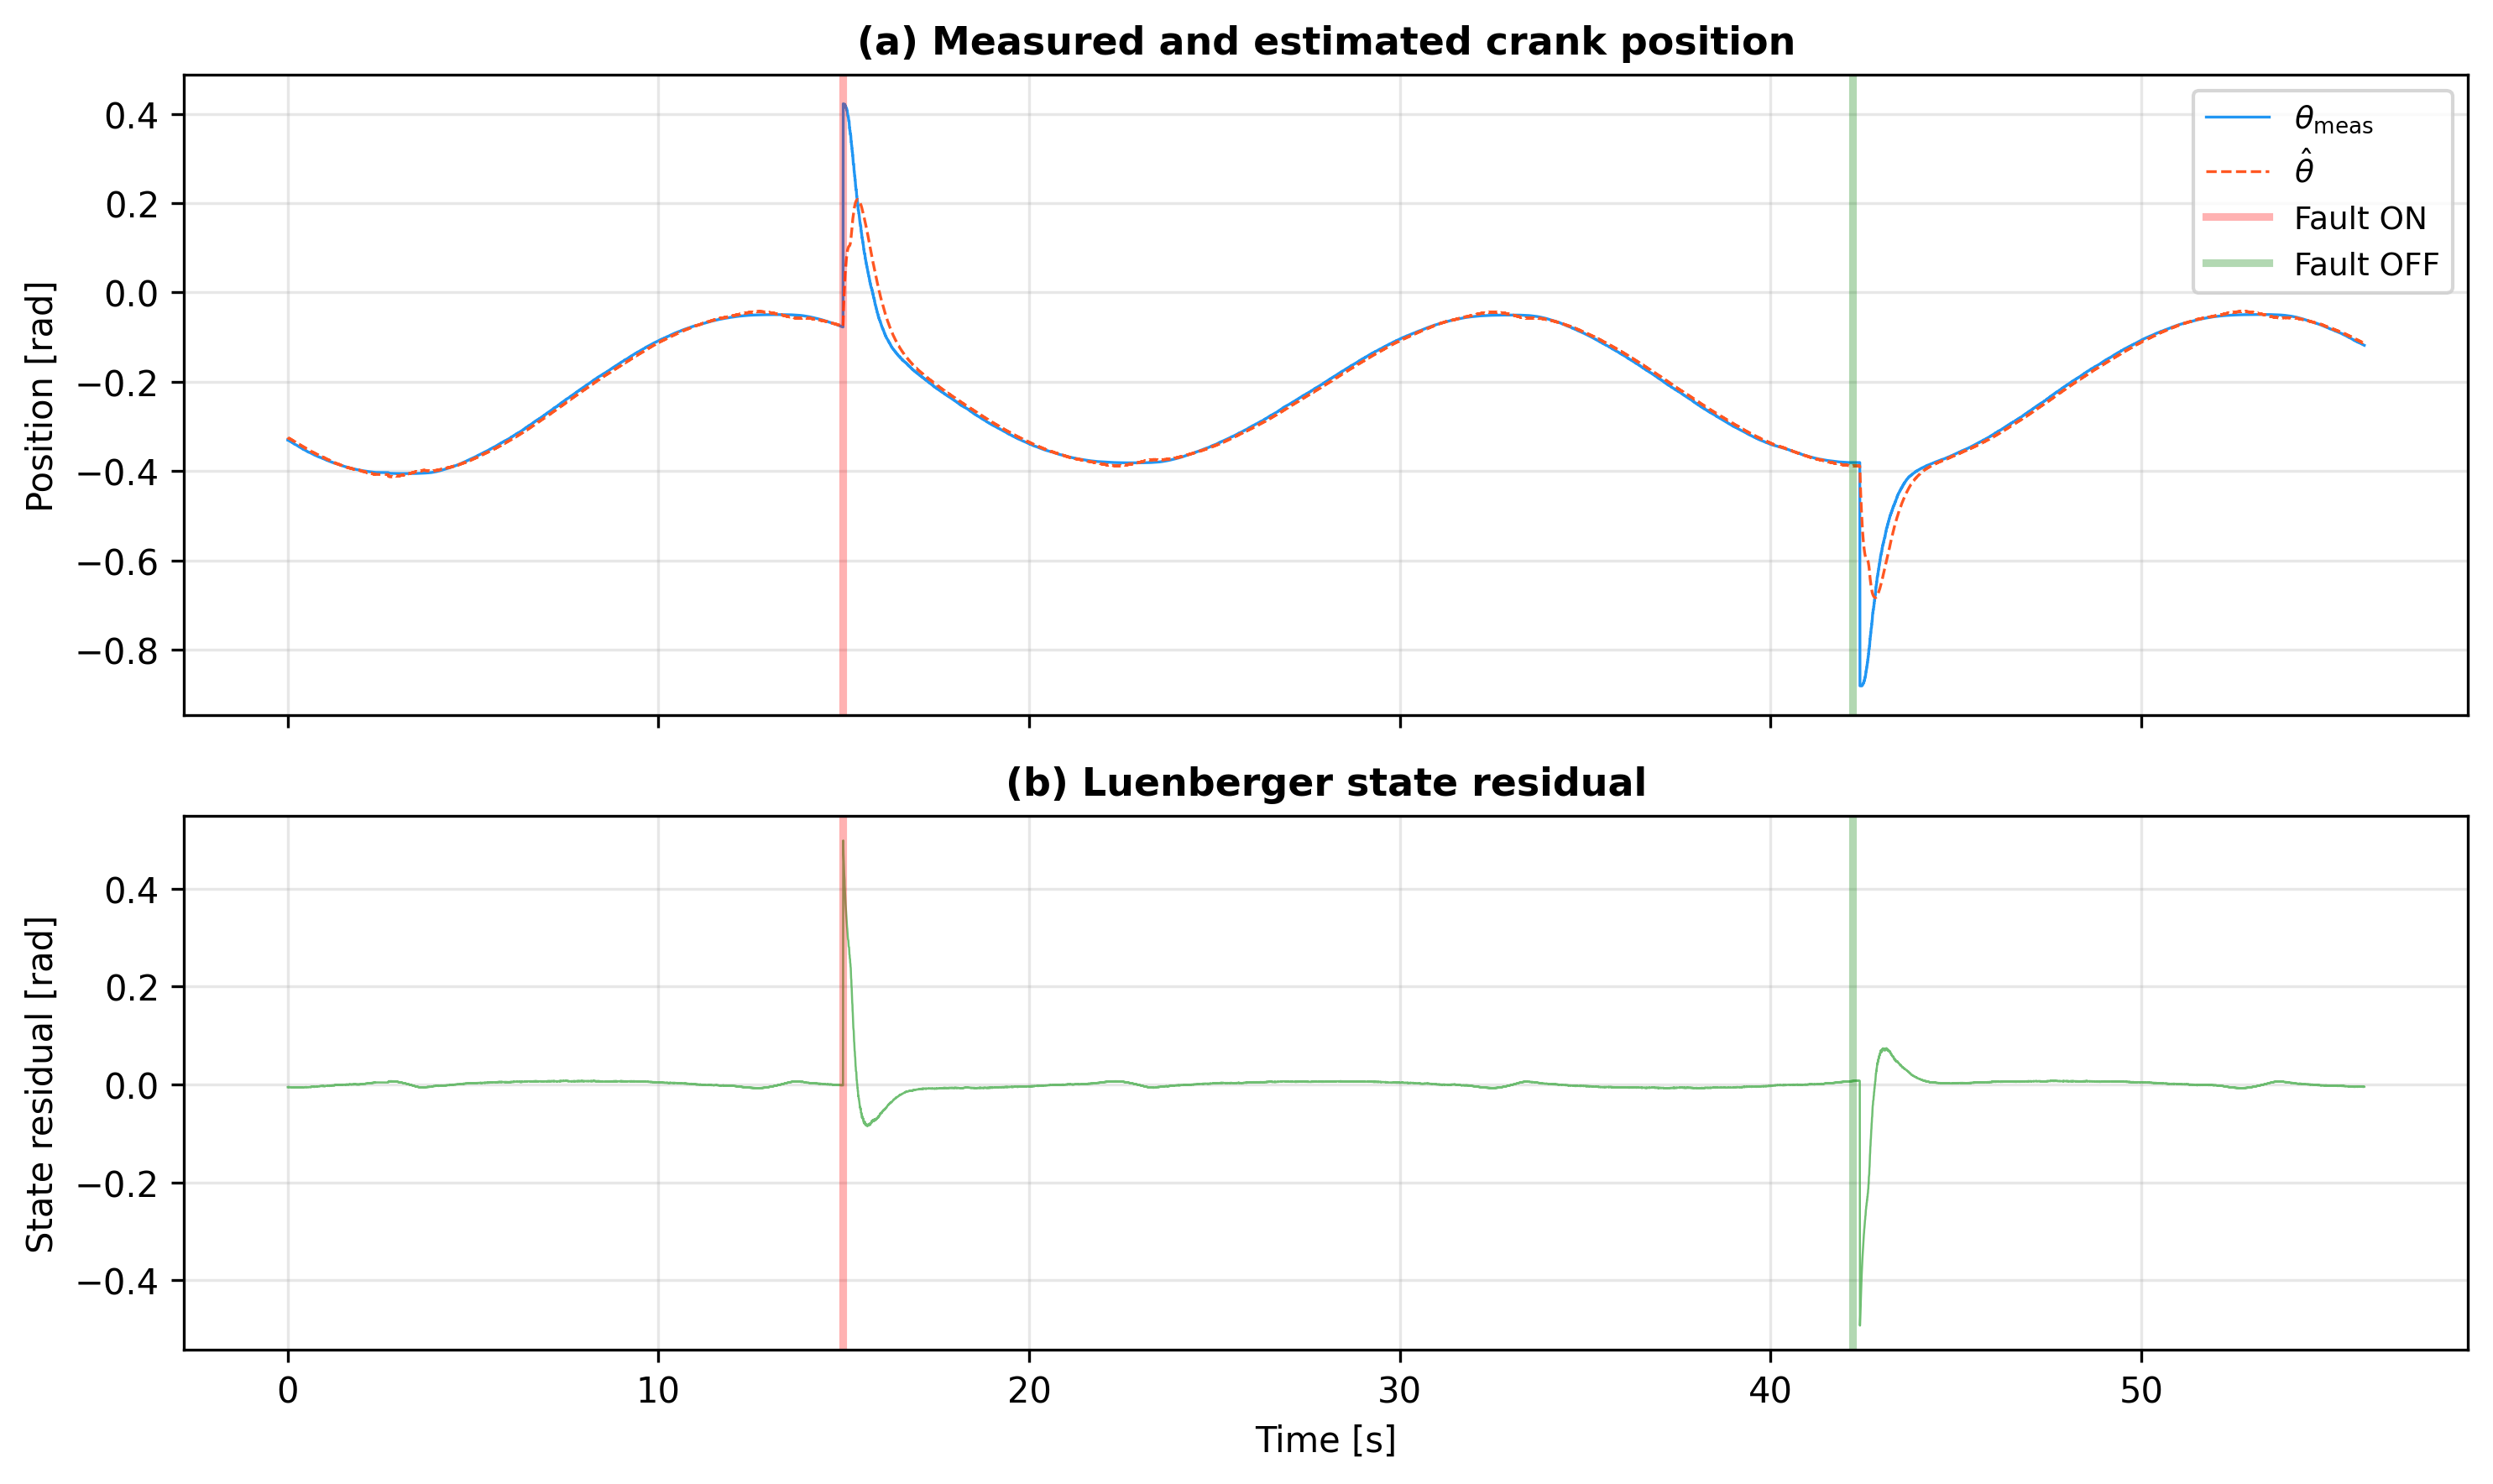
\includegraphics[scale=0.6]{images/chapter6/fig6_3_luenberger_encoder.png}
    \caption{Time-series plot showing the Luenberger state residual in response to a step offset injected on the position encoder.}
    \label{fig:luenberger_residual}
\end{figure}
\FloatBarrier

\subsection{Observer 2 - Admittance Inversion}
The second observer exploits the known structure of the admittance controller (Section 4.4.2) to reconstruct the external force from the trajectory reference signals. If the admittance controller is operating nominally — that is, its virtual dynamics are not saturated — then the relationship between the external force and the reference trajectory is deterministic:

\begin{equation}
    \hat{\tau}_{\text{ext}} = M_v \ddot{\theta}_{\text{ref}} + D_v \dot{\theta}_{\text{ref}} + K_v (\theta_{\text{ref}} - \theta_{\text{eq}})
\end{equation}

where $M_v$, $D_v$, $K_v$, and $\theta_{\text{eq}}$ are the virtual admittance parameters. The **torque residual** is then defined as the difference between the measured external force and the reconstructed estimate:

\begin{equation}
    r_{\text{torque}} = \tau_{\text{ext,meas}} - \hat{\tau}_{\text{ext}}
\end{equation}

Under nominal conditions, this residual is close to zero because the measured external force and the admittance output are consistent. A fault on the external force sensor (channel 0) causes the measured value to diverge from the reconstructed estimate, producing a non-zero residual.
 
A critical aspect of this observer is the management of \textbf{validity conditions}. The admittance inversion is mathematically valid only when the virtual dynamics are not constrained by the saturation limits described in Section 4.2.3. The observer checks three invalidation conditions at every cycle:

\begin{minted}{python}

    ref_pos_saturated = (
    self._theta_ref <= th_min + sat_margin or
    self._theta_ref >= th_max - sat_margin
)
ref_vel_saturated = (
    abs(self._theta_dot_ref) >= dv_max - sat_margin
)
in_deadband = abs(self._tau_ext_meas) < deadband

\end{minted}

If the position reference is near its saturation bounds, or the velocity reference is near its maximum, or the measured force is within the deadband, the inversion is invalid: the admittance output no longer reflects the external force but is instead determined by the saturation logic. In this case, the observer sets the residual to zero and flags the estimate as invalid (\textbf{obs2\_valid} = False), preventing false alarms from a structurally incorrect comparison. The validity flag is published in the debug vector, allowing downstream analysis to exclude invalid intervals.

\subsection{Observer 3 - Generalized Momentum Observer}
The momentum observer implements the formulation described in Section 6.2.3, maintaining an internal integrator $\sigma$ that tracks the expected evolution of the generalized momentum $p = M_{\text{eff}} \cdot \dot{\theta}$. At each cycle, the known torque contributions are summed, the integrator is updated, and the residual is computed as the gain-weighted deviation between the actual momentum and the integrator state:

\begin{minted}{python}

    p_now = self._M_eff * self._theta_dot_meas

tau_known = (
    self._tau_m
    + self._tau_pass
    + self._tau_ext_meas
    - self._proj
    - tau_dissipative_m
)

# Inertia variation compensation
delta_p_M = (self._M_eff - self._M_eff_prev) \
            * self._theta_dot_meas

# Integrator update
self._mom_sigma += \
    (tau_known + self._r_momentum) * dt + delta_p_M

# Residual
self._r_momentum = K_mom * (p_now - self._mom_sigma)

\end{minted}

The term \textbf{delta\_p\_M} compensates for the configuration-dependent variation of the effective inertia $M_{\text{eff}}(\theta)$, which would otherwise appear as a spurious residual whenever the crank moves through regions of varying inertia. This discrete compensation is computed as the product of the inertia change between consecutive steps and the current velocity, and is added directly to the integrator update.
 
The residual $r_{\text{mom}}$ is published on \textbf{/observer/momentum\_residual}. With the default gain $K_{\text{mom}} = 50\,\text{s}^{-1}$, the observer has a time constant of approximately 20 ms, resulting in a detection latency of 40-60 ms for a step fault - an order of magnitude faster than the Luenberger observer for force-related faults. This speed advantage comes from the fact that the momentum observer operates directly on the torque balance, without requiring the fault effect to propagate through the closed-loop dynamics.

\begin{figure}[ht]
    \centering
    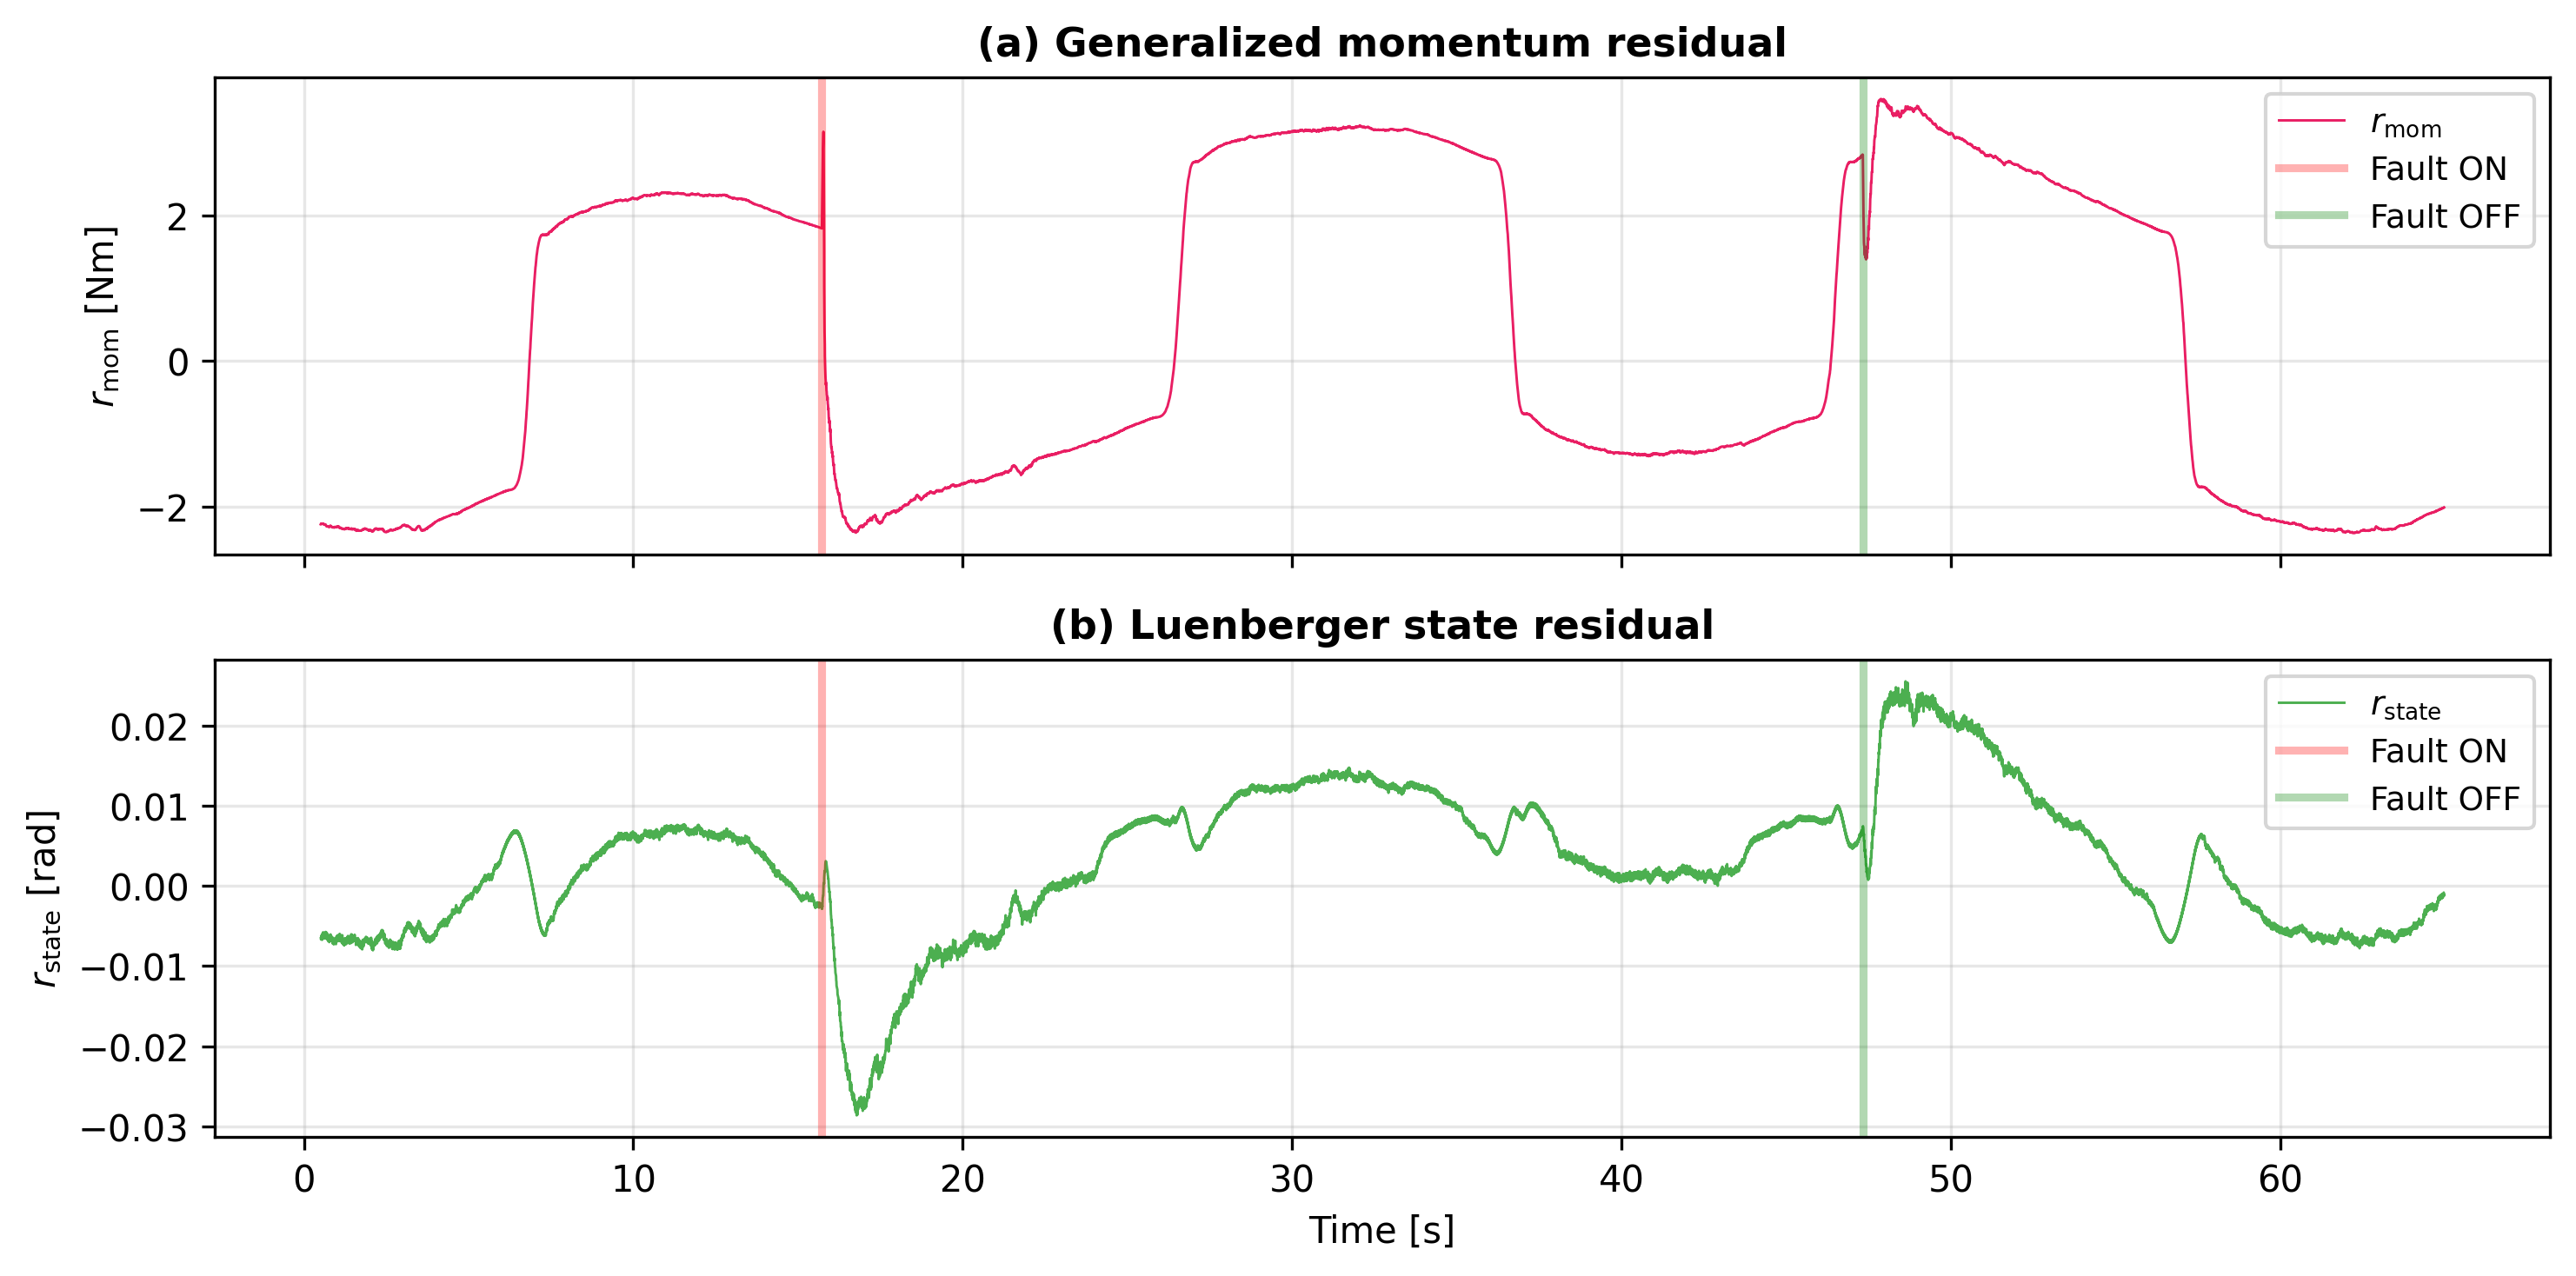
\includegraphics[scale=0.6]{images/chapter6/fig6_4_momentum_vs_luenberger.png}
    \caption{Time-series plot comparing the momentum residual and the Luenberger state residual in response to a step offset fault on the external user force sensor.}
    \label{fig:momentum_vs_luenberger}
\end{figure}
\FloatBarrier

\subsection{Guard 4 - Rate-of-Change Monitor}
The rate-of-change guard computes the discrete derivative of the external force signal at each cycle and compares its absolute value against the physiological limit:

\begin{minted}{python}

    self._tau_ext_rate = abs(self._tau_ext_meas - self._tau_ext_prev) / dt
    self._rate_alarm = self._tau_ext_rate > max_rate
    self._tau_ext_prev = self._tau_ext_meas

\end{minted}

The alarm signal is published on \textbf{/observer/tau\_ext\_rate\_alarm} as a binary value (1.0 if the rate exceeds the threshold, 0.0 otherwise). With the default threshold of 100 Nm/s, the guard triggers on any force discontinuity larger than approximately 0.5 Nm within a single 5 ms sample - well below the magnitude of a typical injected offset fault (2 Nm, corresponding to 400 Nm/s) but well above the maximum physiological rate of force production by the human hand.
 
The primary strength of this guard is its detection latency: exactly one sample (5 ms), the theoretical minimum for any discrete-time detector. Its primary limitation is that it is completely blind to slow drifts — a gradually increasing bias of 0.01 Nm per second, for instance, would never exceed the rate threshold despite eventually reaching a dangerous magnitude. This limitation is complementary to the momentum observer, which detects such drifts but requires a longer observation window.

\subsection{Residual Filtering and Diagnostic Output}
Residuals undergo post-processing via an exponential moving average filter ($\alpha = 0.05$, time constant $\approx 100ms$ at $200Hz$) and a sliding-window RMS computation (50 samples / 250ms) to produce smoothed residuals and a scalar measure of residual energy robust against noise spikes. A 21-field debug vector containing estimated states, measured inputs, raw and filtered residuals, validity flags, and momentum/rate outputs is published each cycle on \textbf{/observer/debug}, serving as the primary data source for offline analysis and threshold calibration.

\begin{figure}[ht]
    \centering
    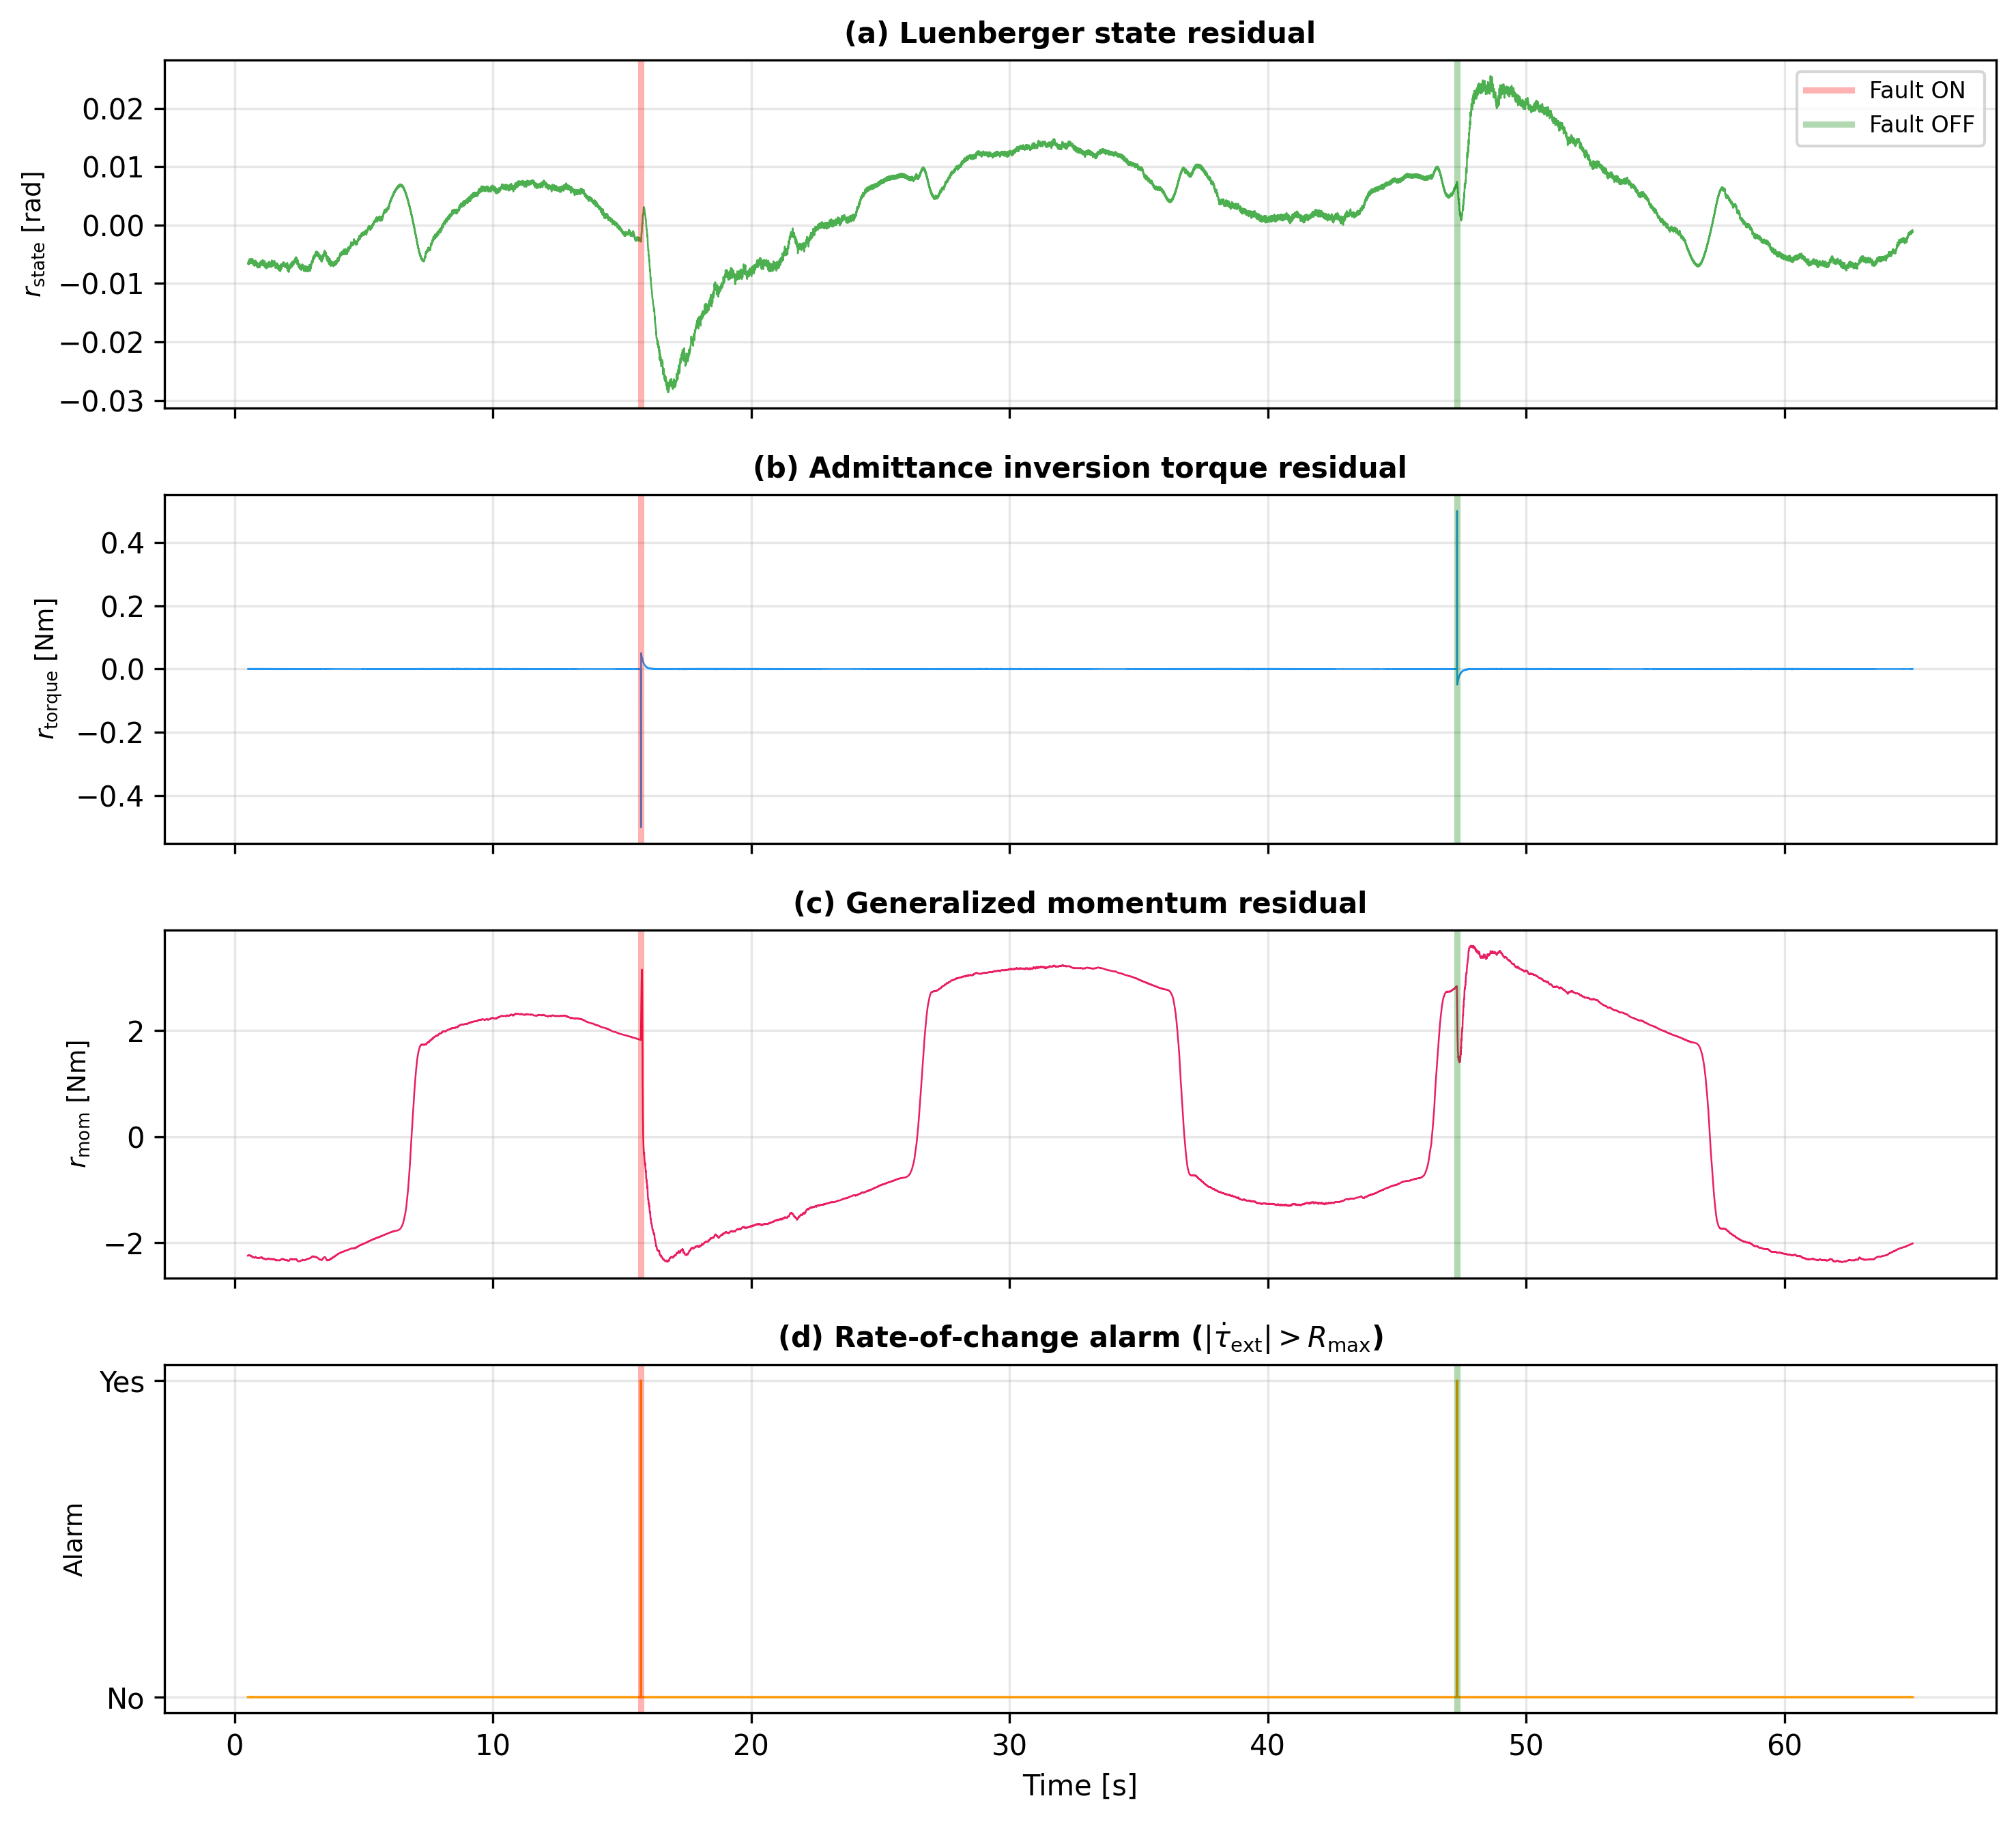
\includegraphics[scale=0.60]{images/chapter6/fig6_5_multipanel_residuals.png}
    \caption{Multi-panel time-series plot showing the four residual signals simultaneously during a fault injection experiment. Panel (a): Luenberger state residual (raw and EMA-filtered). Panel (b): admittance inversion torque residual (with obs2\_valid shading). Panel (c): momentum residual. Panel (d): rate-of-change alarm (binary).}
    \label{fig:multipanel_residuals}
\end{figure}
\FloatBarrier




\section{Sensor Health Assessment}
The four observer layers described in Section 6.3 produce residual signals that are each sensitive to a different subset of the possible fault conditions. When considered in isolation, each residual provides partial information about the health of a specific signal channel; when considered together, they form a diagnostic signature that can, in principle, be used to both detect and isolate faults across the entire sensing and actuation chain of the exoskeleton.

\subsection{Fault Sensitivity Mapping}
Each observer layer has a primary sensitivity - the fault type to which it responds most strongly and with the shortest latency - and one or more secondary sensitivities - fault types that produce a detectable but weaker or delayed response. This mapping is summarized in Table 6.1.

\begin{table}[H]
\centering
\small
\caption{Fault sensitivity matrix: residual latencies for different observer types and fault channels.}
\label{tab:observer_latencies}
\begin{tabularx}{\textwidth}{l*{4}{>{\centering\arraybackslash}X}}
\toprule
\textbf{Observer} & \textbf{Ch.\,0 ($\tau_{\text{ext}}$)} & \textbf{Ch.\,1 (traj.\ ref)} & \textbf{Ch.\,2 (torque)} & \textbf{Ch.\,3 (encoder)} \\
\midrule
Luenberger       & secondary, $\sim$1--1.5\,s              & secondary, $\sim$1\,s        & secondary, $\sim$0.5\,s  & \textbf{primary}, $\sim$10\,ms  \\
Admittance Inv.  & \textbf{primary}, $\sim$50\,ms           & secondary, $\sim$20\,ms      & ---                      & ---                             \\
Momentum         & \textbf{primary}, $\sim$40--60\,ms       & ---                          & secondary, $\sim$50\,ms  & secondary, $\sim$100\,ms        \\
Rate-of-Change   & \textbf{primary}\textsuperscript{**}, $\sim$5\,ms & ---               & ---                      & ---                             \\
\bottomrule
\end{tabularx}
\vspace{4pt}
{\footnotesize \textsuperscript{**}Impulsive faults only.}
\end{table}
\FloatBarrier

The table reveals the complementary nature of the four layers. No single observer covers all four channels with the same effectiveness, but the combination provides at least one primary detector for each channel.
 
The \textbf{encoder channel} (Ch. 3) is primarily covered by the Luenberger observer, which detects position and velocity corruption directly through the innovation signal. An encoder fault also affects the momentum observer since $p = M_{\text{eff}} \cdot \dot{\theta}_{\text{meas}}$ depends on the measured velocity, but the effect is indirect and more difficult to distinguish from a torque-related fault.
 
The \textbf{external force channel} (Ch. 0) has triple coverage. The rate-of-change guard provides the fastest response (one sample) for impulsive faults such as sudden offsets or spikes. The momentum observer provides fast detection (~40--60 ms) for both impulsive and sustained faults, including slow drifts that are invisible to the rate guard. The admittance inversion provides an independent cross-check by reconstructing the force from the trajectory reference, but is available only when the admittance controller is not saturated.
 
The \textbf{torque channel} (Ch. 2) is primarily covered by the momentum observer, which detects discrepancies in the torque balance. The Luenberger observer provides secondary coverage with a longer latency, as the torque fault must first affect the crank motion before it becomes visible in the position innovation.
 
The \textbf{trajectory reference channel} (Ch. 1) has the weakest coverage in the current implementation. The admittance inversion provides partial sensitivity - a corrupted trajectory reference produces an inconsistency between the measured force and the reconstructed estimate - but the detection is indirect and depends on the operating conditions. This channel represents the most significant gap in the current observer architecture and is discussed further in Section 6.5.

\subsection{Detection Latency Spectrum}
A distinctive feature of the multi-observer architecture is the range of detection timescales it covers. The four layers span three orders of magnitude in detection latency:

\begin{itemize}
    \item \textbf{5 ms} (1 sample): the rate-of-change guard, for impulsive faults on the external force;
    \item \textbf{4-60 ms}: the momentum observer, for sustained faults on the torque balance;
    \item \textbf{50 ms}: the admittance inversion, for force sensor faults (when valid);
    \item \textbf{0.5-1.5 s}: the Luenberger observer, for faults that propagate indirectly through the closed-loop dynamics.
\end{itemize}


This spectrum is significant from a safety perspective. The fastest layers (rate-of-change and momentum) can detect faults well within the control loop bandwidth, enabling, in a future integrated version, a protective response before the fault has time to produce a significant mechanical effect on the user. The slower Luenberger observer, while less useful for rapid fault detection, provides a redundant check that can confirm or refute the alarm raised by the faster observers, reducing the risk of false positives.

\subsection{Nominal Residual Behavior}
An important practical consideration for any observer-based fault detection system is the behavior of the residuals under nominal conditions. A residual that is perfectly zero in theory will, in practice, exhibit a non-zero baseline due to modeling uncertainties, numerical integration errors, and measurement noise. The magnitude of this nominal baseline determines the minimum detectable fault: any fault whose effect on the residual is smaller than the baseline level will be indistinguishable from normal operation.
 
In the current implementation, the nominal residual levels observed during fault-free Digital Twin simulations are:

\begin{itemize}
    \item \textbf{Luenberger state residual}: on the order of $10^{-4}$ rad, dominated by the discretization error of the explicit Euler integrator and the mismatch between the observer's friction model (evaluated on $\dot{\hat{\theta}}$) and the plant's friction model (evaluated on $\dot{\theta}$).
    \item \textbf{Admittance inversion residual}: on the order of $10^{-2}$ Nm when valid, primarily due to the EMA filter lag and the discrete-time approximation of the virtual dynamics.
    \item \textbf{Momentum residual}: on the order of $10^{-2}$ Nm, dominated by the inertia variation compensation error and the friction model uncertainty.
    \item \textbf{Rate-of-change}: typically below 20 Nm/s under nominal conditions, well below the 100 Nm/s threshold.
\end{itemize}

These nominal levels provide a baseline against which detection thresholds could be calibrated. However, as discussed in the following section, this calibration has not yet been performed systematically and remains as future work.


\section{Current Status and Integration Outlook}
This section summarizes the current maturity level of the observer module, identifies the work that remains to be done for its integration into the functional safety chain, and outlines the envisioned integration path.

\subsection{Current Status}
The observer node is fully implemented and operational within the Digital Twin. It is deployed as a standard ROS 2 node (\textbf{observer\_node}) with a registered entry point, a dedicated parameter file (\textbf{observer\_params.yaml}), and integration into launch configurations. When launched alongside the plant, controllers, and safety nodes, the observer subscribes to the relevant topics, computes all four residuals at 200 Hz, and publishes them in real time on six dedicated topics plus a comprehensive 21-field debug vector.

The observer has been tested \textbf{qualitatively} in conjunction with the fault injection framework described in Chapter 5. By injecting known faults on each of the four channels and examining the residual responses, the following behaviors have been verified: (i) the Luenberger state residual responds promptly to encoder faults (channel 3); (ii) the momentum residual responds rapidly to force sensor offsets (channel 0) and torque faults (channel 2); (iii) the admittance inversion residual detects force sensor faults when the admittance controller is not saturated; and (iv) the rate-of-change guard triggers immediately on impulsive faults.

The topic remapping in the launch file is configured to ensure that the observer receives the correct signals for each fault injection scenario. For instance, when a fault is injected on channel 0 ($\tau_{ext}$), the observer is remapped to receive the faulted signal so that it can detect the discrepancy, while the plant model terms (
ff\_terms) continue to arrive from the nominal dynamics node. This careful routing ensures that the observer's detection capability is exercised under realistic conditions.

\subsection{What Is Missing for Integration}
Despite being functionally complete as a residual generator, the observer module is not yet connected to the safety decision chain. The gap between the current state and a fully integrated fault detection system can be decomposed into four specific items.

\textbf{Threshold calibration}. The residuals are currently published as continuous signals without any associated detection threshold. To produce a binary fault/no-fault decision, each residual would need a calibrated threshold — or, more robustly, an adaptive threshold that accounts for the operating-point-dependent variation of the nominal residual level. The nominal residual magnitudes reported in Section 6.4.3 provide a starting point for this calibration, but a systematic characterization across the full operating envelope of the mechanism has not yet been performed.

\textbf{Decision logic}. Even with calibrated thresholds, a threshold crossing on a single residual should not directly trigger a safety transition. A proper decision logic would need to account for debouncing (analogous to the mechanism described in Section 5.4.2), confirmation across multiple observers (to reduce false positive rates), and the distinction between transient threshold violations and sustained faults. Statistical methods such as the Cumulative Sum (CUSUM) test or the Generalized Likelihood Ratio (GLR) test are well suited for this purpose but have not yet been implemented.

\textbf{Fault isolation}. The current observer architecture can detect that a fault is present, but it cannot unambiguously identify which sensor is faulty in all cases. The fault sensitivity matrix of Table 6.1 shows that some fault types produce responses in multiple observers, which in principle enables isolation through structured residual analysis. However, the isolation logic — which would map residual patterns to specific fault hypotheses — has not been designed or validated.

\textbf{Service interface}. Once a fault is detected and (optionally) isolated, the observer would need to communicate this information to the safety state machine through the existing ROS 2 service interface. This could follow the same pattern used by the FaultMonitorMode plugin: asynchronous service calls to /\textbf{compliant\_mode\_req}, \textbf{/torque\_limit\_req}, or \textbf{/safe\_stop\_req}, depending on the severity of the detected fault.

\subsection{Integration Path: SENSOR\_DEGRADED\_MODE}
The safety state machine described in Chapter 5 already reserves a fifth safety state - \textbf{SENSOR\_DEGRADED\_MODE} - in its SafetyState enumeration (Section 5.3.1). This state is not currently reachable through any transition path, but it was included in the design precisely to accommodate the future integration of the observer module.

The envisioned integration path is as follows. The observer node would be extended with a threshold evaluation and decision logic layer that produces a fault diagnosis. When a sensor fault is confirmed with sufficient confidence, the observer would call a new service - for instance, \textbf{/sensor\_degraded\_request} - on the state machine, requesting a transition to \textbf{SENSOR\_DEGRADED\_MODE}. The state machine would need a minor extension to register this service and to add the corresponding transition rules to the \textbf{can\_transition\_to()} method. A new plugin, SensorDegradedMode, would implement the appropriate bridge mode for degraded-sensor operation, for instance, switching to an observer-based state estimate for the feedback loop while maintaining reduced control authority.

This integration path requires no architectural changes to the existing safety framework: the plugin-based design, the service interface, and the bridge mode system are already in place. The primary effort lies in the calibration, decision logic, and validation work described above, tasks that are well defined but require dedicated experimental campaigns on the physical prototype or on a high-fidelity Digital Twin simulation that includes realistic sensor noise models.

\subsection{Directions for Improvement}
Beyond the integration items described above, several technical improvements could enhance the robustness and diagnostic capability of the observer module:

\textbf{Adaptive thresholding}. The nominal residual level varies with the operating point, in particular, with the crank velocity and the magnitude of the passive biomechanical torques. A fixed threshold that is tight enough to detect small faults at low velocity may produce false alarms during fast motion. An adaptive threshold that scales with the instantaneous operating conditions would provide a more uniform detection sensitivity across the workspace.

\textbf{Observer fusion}. The four residuals are currently independent signals with no cross-correlation analysis. A fusion layer — for instance, a weighted voting scheme or a Bayesian classifier — could combine the evidence from multiple observers to produce a single, more robust fault indicator with a lower false positive rate than any individual residual.

\textbf{Parametric robustness analysis}. The observer performance depends on the accuracy of the plant model parameters, particularly the friction coefficients and the effective inertia. A formal sensitivity analysis — quantifying how much each parameter uncertainty contributes to the nominal residual level — would provide guidance for robust threshold design and would identify the parameters that most critically require accurate identification.

\textbf{Online parameter adaptation}. In a future hardware-in-the-loop deployment, the plant parameters may drift over time due to wear, temperature changes, or variations in the user's hand properties. An online parameter estimation layer could track these variations and update the observer model accordingly, maintaining detection sensitivity over extended operating periods.

\section{Summary}
This chapter has presented the model-based fault detection module developed for the hand exoskeleton Digital Twin, covering the theoretical foundations, the implementation of four complementary observer layers, and the current status of the work.

The observer node implements a Luenberger state observer for encoder fault detection, an admittance inversion estimator for external force sensor monitoring, a generalized momentum observer for fast torque-balance discrepancy detection, and a rate-of-change guard for instantaneous identification of impulsive signal corruptions. Together, the four layers provide coverage across all four critical signal channels of the control architecture, with detection latencies spanning from 5 ms (one sample) to approximately 1.5 seconds depending on the observer type and the fault propagation path.

The module is fully operational within the Digital Twin: it runs at 200 Hz alongside the plant and control nodes, publishes residuals and diagnostic information in real time, and has been qualitatively validated using the fault injection framework of Chapter 5. However, the observer is not the primary focus of this thesis and has not yet been connected to the functional safety decision chain. The residuals are currently published for monitoring and offline analysis purposes only.

The integration path toward a complete model-based fault detection and mitigation system is well defined and leverages the extensible architecture of the safety state machine described in Chapter 5. The \textbf{SENSOR\_DEGRADED\_MODE} state, already reserved in the safety state enumeration, provides the natural entry point for observer-triggered protective actions. The remaining work (threshold calibration, decision logic design, and systematic validation) constitutes a clearly scoped future effort that can build directly on the infrastructure developed in this thesis.